\chapter{Progettazione concettuale}
		\section{Class Diagram}	
	\begin{SCfigure}[50][h]

	\centering
	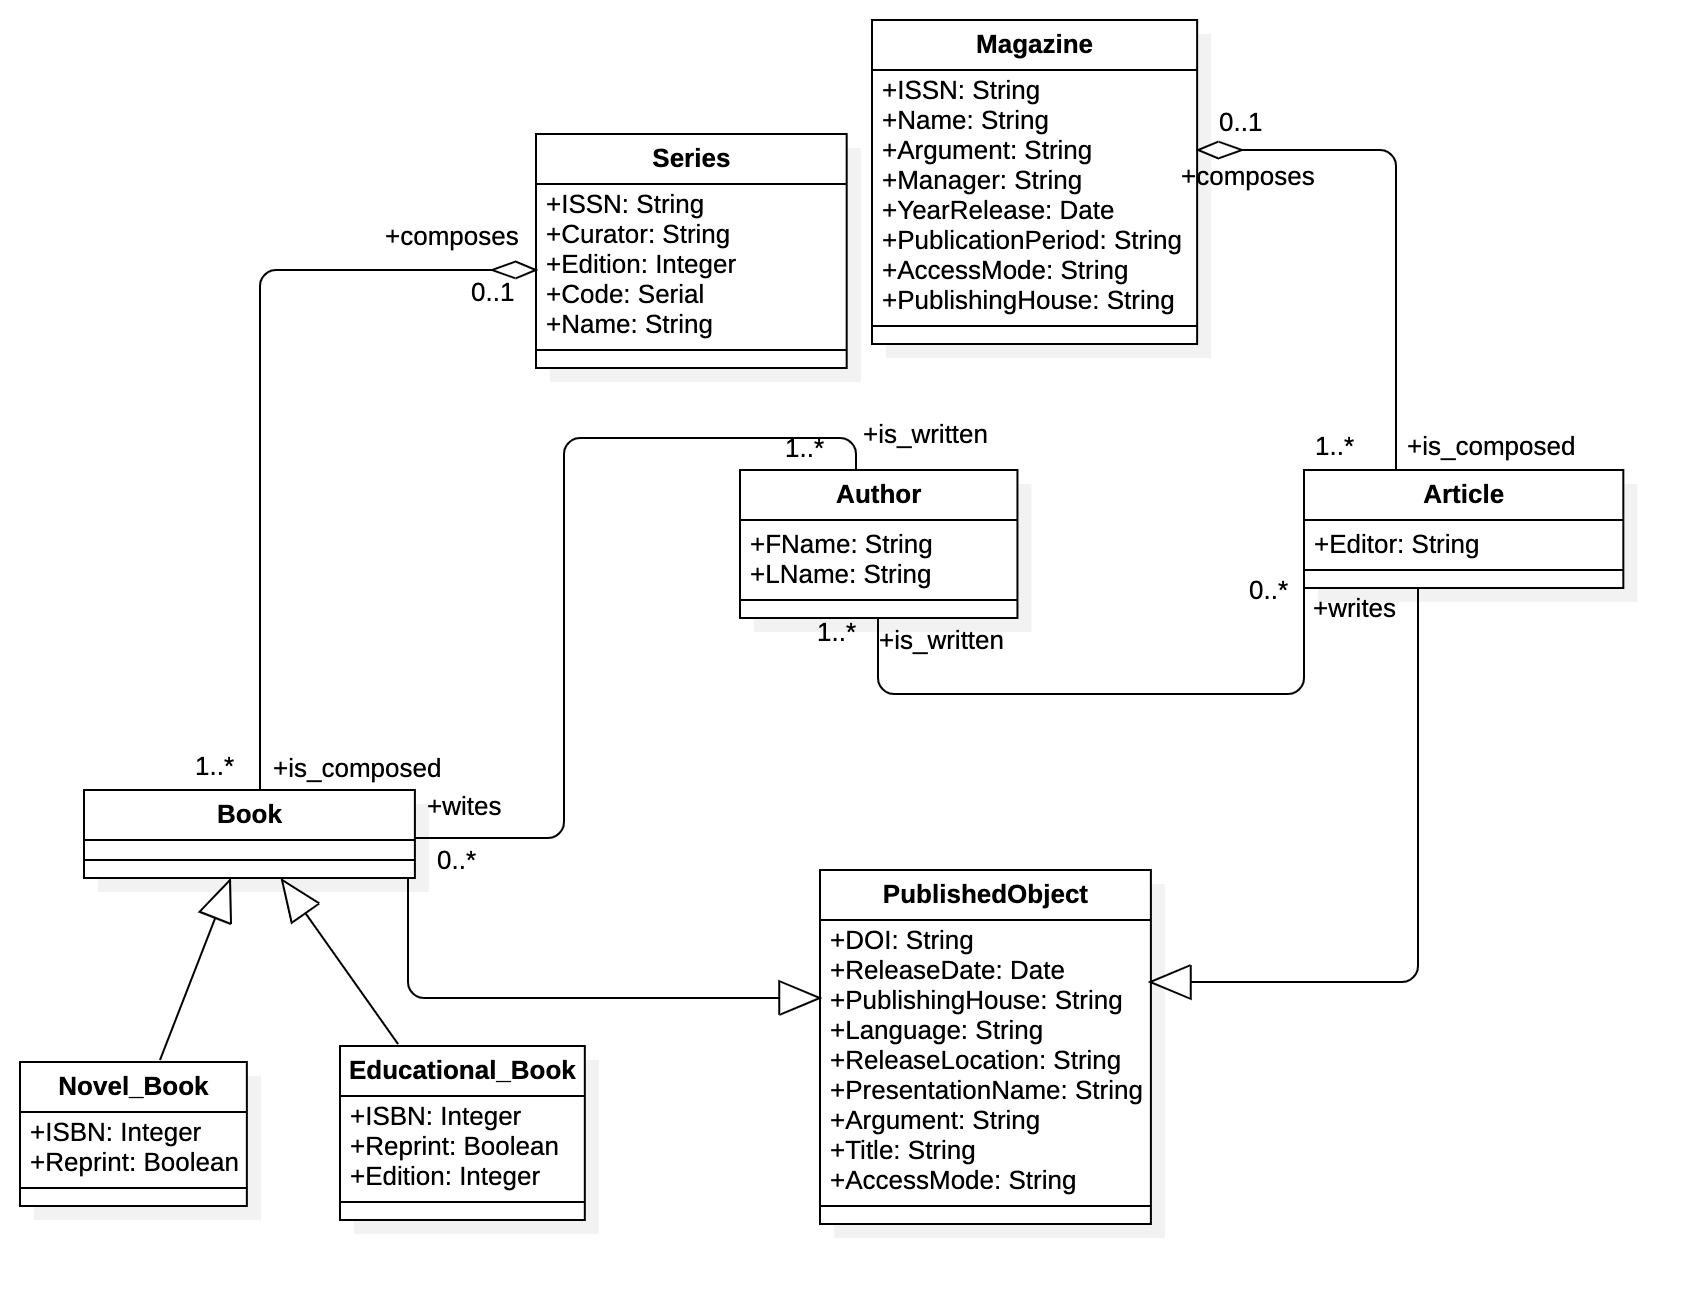
\includegraphics[width=0.8\textwidth]{Immagini/ClassDiagram.png}
	\caption{Class Diagram}
	\label{fig:ClassDiagram}
	\end{SCfigure}

    \section{Analisi della ristrutturazione del Class Diagram}
        
        \subsection{Analisi delle ridondanze}
            
        \subsection{Analisi degli identificativi}
            
        \subsection{Rimozione degli attributi multipli}
            
        \subsection{Rimozione degli attributi composti}
            
        \subsection{Partizione/Accorpamento delle associazioni}
            
        \subsection{Rimozione delle gerarchie}
    
    \section{Class Diagram ristrutturato}
  
    \begin{SCfigure}[50][h]

	\centering
	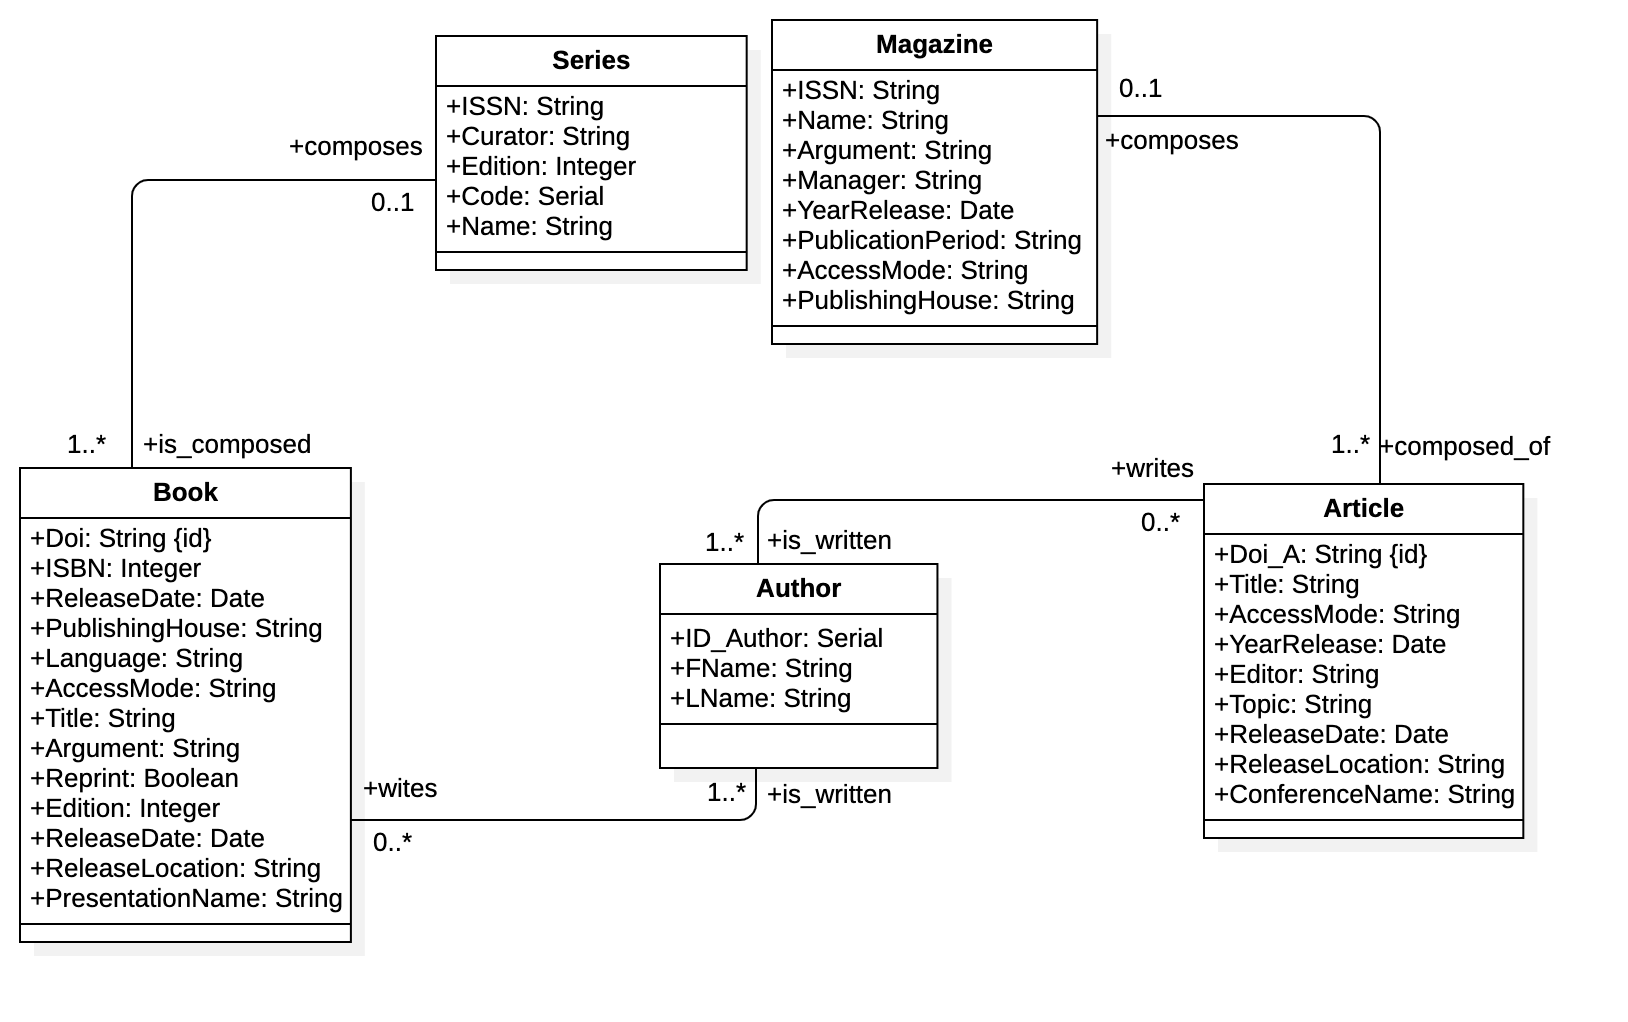
\includegraphics[width=0.8\textwidth]{Immagini/ClassDiagramRIS.png}
	\caption{Class Diagram \\ Ristrutturato}
	\label{fig:ClassDiagramRIS}
	\end{SCfigure}

\newpage
\section{Dizionario delle classi}
	


\begin{longtable}{l|l|l} 
\caption{Dizionario delle Classei}
\\
Class    & Explanation                                                                                                                                                & Attributes                                                                                                                                                                                                                                                                                                                                                                                                                                                                                                                                                                                                                                                                                                                                                                                                                                                                                                                                                                                                                                                                                                                                                                                                                                                                                                                     \\ 
\hline
Authors  & \textcolor[rgb]{0.125,0.129,0.141}{Authors of books or articles}                                                                                           & \multicolumn{1}{l}{\begin{tabular}[c]{@{}l@{}}\\\\ID\_Author (Serial): Author's \\identification code\\FName (String): Author's first \\ name\\LName (String):~Author's last \\ name\\\\\\\\\end{tabular}}                                                                                                                                                                                                                                                                                                                                                                                                                                                                                                                                                                                                                                                                                                                                                                                                                                                                                                                                                                                                                                                                                                                             \\ 
\cline{1-2} \hline
Book     & \begin{tabular}[c]{@{}l@{}}\textcolor[rgb]{0.125,0.129,0.141}{Books that can be novels }\\\textcolor[rgb]{0.125,0.129,0.141}{or educational~}\end{tabular} & \begin{tabular}[c]{@{}l@{}}\\\\DOI~(String): Digital object Identifier\\of the book.\\ISBN (Integer):~\textcolor[rgb]{0.125,0.129,0.141}{Numerical classification}\\\textcolor[rgb]{0.125,0.129,0.141}{sequence of the book.}\\Edition~(Integer):~\textcolor[rgb]{0.125,0.129,0.141}{Edition number.}\\AccessMode (AccessMode): Fruition\\method.\\ReleaseDate (Date):~\textcolor[rgb]{0.125,0.129,0.141}{Publication date.}\\PublishingHouse (String):~\textcolor[rgb]{0.125,0.129,0.141}{Publishing }\\\textcolor[rgb]{0.125,0.129,0.141}{house}\\\textcolor[rgb]{0.125,0.129,0.141}{that printed the book.}\\ReleaseLocation (String):~\textcolor[rgb]{0.125,0.129,0.141}{Place of }\\\textcolor[rgb]{0.125,0.129,0.141}{publication}\\\textcolor[rgb]{0.125,0.129,0.141}{of the book.}\\Language (String):~\textcolor[rgb]{0.125,0.129,0.141}{Language in which}\\\textcolor[rgb]{0.125,0.129,0.141}{the book}\\\textcolor[rgb]{0.125,0.129,0.141}{is written.}\\Title (String): Book title.\\Argument (String): Book topic.\\Reprint (Boolean):~\textcolor[rgb]{0.125,0.129,0.141}{Parameter that}\\\textcolor[rgb]{0.125,0.129,0.141}{identifies}\\\textcolor[rgb]{0.125,0.129,0.141}{if the book is a reprint or not.}\\PresentationName (String): Name of \\pesentation in which books are presented\\\\\\\end{tabular}  \\ 
\hline
Series   & \textcolor[rgb]{0.125,0.129,0.141}{Set of books~}                                                                                                          & \begin{tabular}[c]{@{}l@{}}\\\\ISSN (Integer):~\textcolor[rgb]{0.125,0.129,0.141}{International number}\\\textcolor[rgb]{0.125,0.129,0.141}{that identifies serial publications.}\\Edition (Integer):~\textcolor[rgb]{0.125,0.129,0.141}{Edition number.}\\Curator (String):~\textcolor[rgb]{0.125,0.129,0.141}{Curator of the series}.\\Code (Serial):~\textcolor[rgb]{0.125,0.129,0.141}{Code assigned to the }\\\textcolor[rgb]{0.125,0.129,0.141}{series.}\\Name (String): Series' name .\\\\\\\\\end{tabular}                                                                                                                                                                                                                                                                                                                                                                                                                                                                                                                                                                                                                                                                                                                                                                                                             \\ 
\hline
Magazine & \textcolor[rgb]{0.125,0.129,0.141}{Set of articles}                                                                                                        & \begin{tabular}[c]{@{}l@{}}\\\\ISSN (Integer):~\textcolor[rgb]{0.125,0.129,0.141}{International number }\\\textcolor[rgb]{0.125,0.129,0.141}{that}\\\textcolor[rgb]{0.125,0.129,0.141}{identifies serial publications.}\\Name (String): Magazine's name\\Argument (String): Magazine topic.\\Manager (String):~\textcolor[rgb]{0.125,0.129,0.141}{Event organizer.}\\YearRelease (Date):~\textcolor[rgb]{0.125,0.129,0.141}{Publication year.}\\PublicationPeriod (String):~\textcolor[rgb]{0.125,0.129,0.141}{Periodicity}\\\textcolor[rgb]{0.125,0.129,0.141}{of publication.}\\AccessMode (AccessMode): Fruition\\method.\\\\\\\end{tabular}                                                                                                                                                                                                                                                                                                                                                                                                                                                                                                                                                                                                                                                                                \\ 
\hline
Article  & \textcolor[rgb]{0.125,0.129,0.141}{Articles of~ scientific research}                                                                                       & \begin{tabular}[c]{@{}l@{}}\\\\DOI (String): Digital object Identifier \\of the book.\\Title (String): Book title.\\AccessMode (AccessMode): Fruition method.\\YearRelease (Date):~\textcolor[rgb]{0.125,0.129,0.141}{Publication year.}\\Editor (String):\textcolor[rgb]{0.125,0.129,0.141}{Article editor.}\\ReleaseDate (Date):~\textcolor[rgb]{0.125,0.129,0.141}{Publication date.}\\ReleaseLocation (String):~\textcolor[rgb]{0.125,0.129,0.141}{Place of}\\\textcolor[rgb]{0.125,0.129,0.141}{publication}\textcolor[rgb]{0.125,0.129,0.141}{of the book.}\\ConferenceName (String): Name of \\pesentation in which books are presented\textcolor[rgb]{0.125,0.129,0.141}{}\end{tabular}                                                                                                                                                                                                                                                                                                                                                                                                                                                                                                                                                                                                                                      \\
\hline
\end{longtable}


\newpage
\section{Dizionario delle associazioni}
